\documentclass[12pt,a4paper]{article}

\usepackage{amsmath}
\usepackage{physics}
\usepackage[utf8]{inputenc}
\usepackage{graphicx}
\usepackage{biblatex}
\usepackage{float}
\usepackage{caption}
\usepackage{subcaption}

% TODOS WHEN DONE:
%   - Feynman diagrams
%   - Hyperref
%   - Abstract
%   - Fix first plots in data analysis
%   - Discussion
%   - Error + Errorbars
%   - Conclusion
%   - Titlepage
%   - Update (maybe fix) fit to delphes data
%   - Delphes track stuff?

\addbibresource{References.bib}
\nocite{*}

\numberwithin{equation}{section}

\begin{document}

TITLE\\
AUTHORS\\
DATE

\cleardoublepage{}
\begin{abstract}
  
\end{abstract}
\cleardoublepage{}
\tableofcontents{}
\cleardoublepage{}
\section{Introduction}
The standard model (SM) of particle physics is very successful at describing the
fundamental constituents of matter in our universe. Through experiments with
particle accelerators, many of the theoretical details in the SM has been
corroborated. To further test the theory larger accelerators are needed, which
led to the construction of the large hadron collider (LHC), finished in 2008.
Particles are collided together at high energy to probe the properties of the
produced debris, hoping to discover new physics that deviates from the SM.\\

The top quark was discovered in 1995, by experiments done by CDF\cite{Abe_1995}
and DØ\cite{Abachi_1995}. It is the heaviest known fundamental particle, with a
mass of $173.34 \pm 0.27 \pm 0.71 \mathrm{GeV/c^2}$, and its coupling strength
to all the bosons are well predicted by the standard model. Because of its heavy
mass and consequently short lifetime, it doesn't have enough time to bind with
lighter quarks and form hadrons before it decays, which means that it
effectively decays, to a good approximation, as a free quark. Measurements of
the top quark's properties plays an important role in testing the Standard
Model. Top quark production at LHC occurs via strong interactions, where they
are produced in top, anti-top pairs. One test of the Standard Model, is the
study of the $Wtb$ vertex Lorentz structure and coupling, which is studied by
looking at the decay products of top quarks. The top quarks decay, with almost
100\% branching fraction, by weak interactions into $W$ bosons and bottom quarks
$t \rightarrow W + b$. The $W$ bosons decay, into either a charged lepton
and neutrino; $W \rightarrow l + \nu_l$, or into a quark, anti-quark pair: $W \rightarrow q' + \bar{q}$.\\

\begin{figure}[H]
	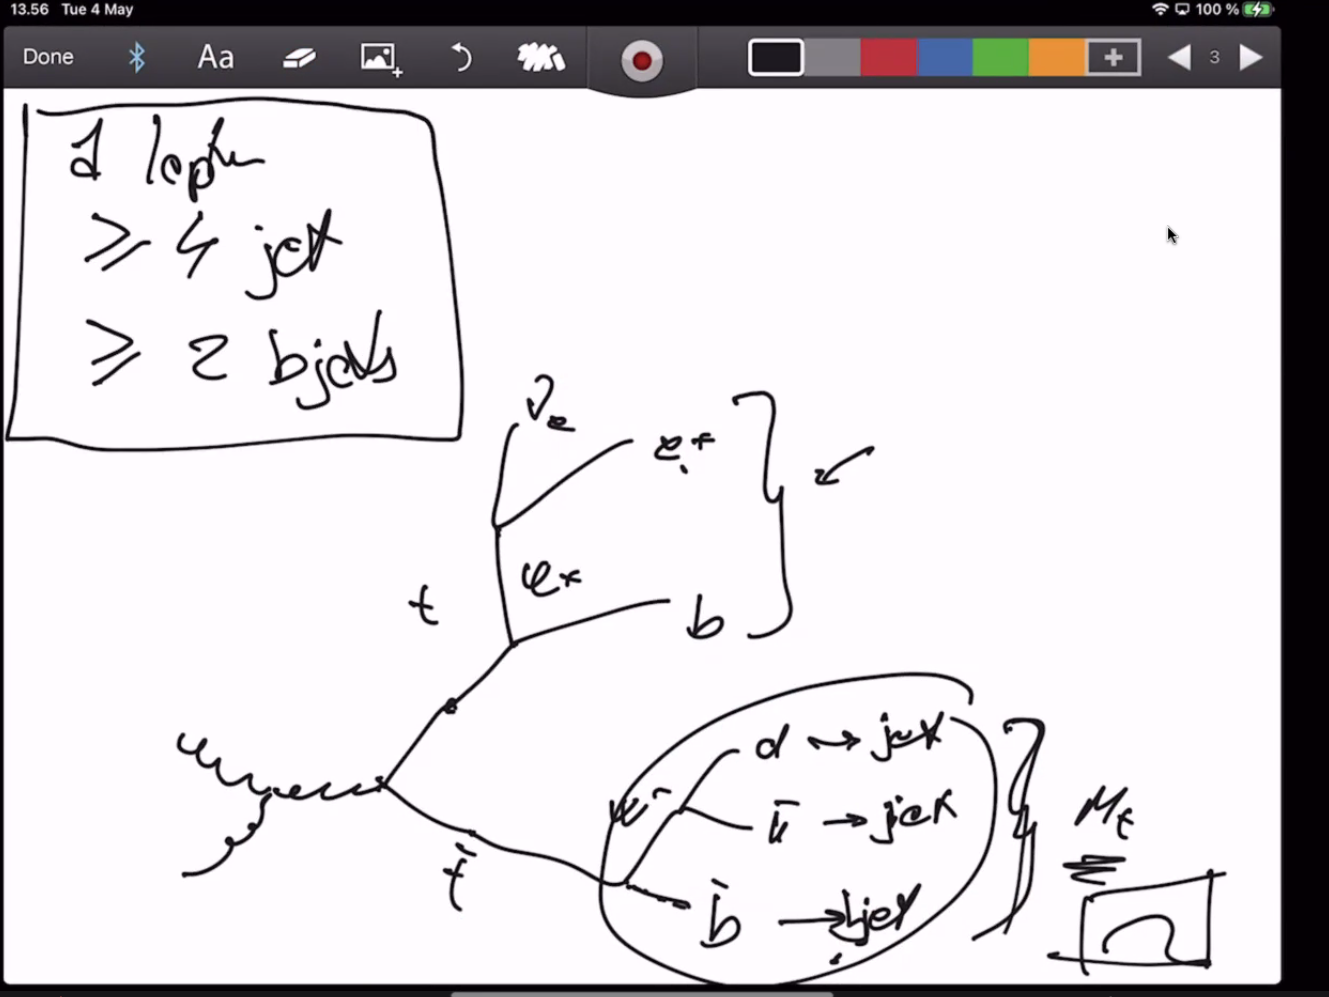
\includegraphics[width=\linewidth]{Placeholder_FeynmanDiagram.png}
	\caption{The Feynman diagram shows one of the possible decays of the top
      quarks. For this single leptonic decay, we see from the figure that there
      are 4 quark jets as the end product.}\label{figfeynmandiagram}
\end{figure}

In this report, we are only looking at decays with a single lepton as decay
product. The leptons we look at are either electrons or muons, and the collision
will produce four jets, as evident from the diagram.

\section{Theory}

\subsection{Standard Model}
The Standard Model is a relativistic quantum field theory that describes three
of the four fundamental forces, (the electromagnetic force, the strong force and
the weak force), into a single theoretical framework. It contains all the known
elementary particles, and how these particles interact with the different
fields. The standard model manages to unify the electromagnetic (EM), and the
weak force into different aspects of the same force called the electroweak
force, while describing strong interactions through the framework of Quantum
Chromodynamics.\\

The elementary particles can be split into two distinct categories, called
fermions and bosons. Fermions are defined by their spin, which is a half odd
integer spin, but is exclusively $1/2$ for all the elementary fermions of the
Standard Model. They obey the pauli-exclusion principle which means that two
identical fermions can't occupy the same quantum state. The fermions are grouped
into quarks and leptons, each with three generations or families based on their
masses. All of the fermions have an antiparticle associated with them, each with
opposite charge, and apart from these antiparticle partners, there are a total
of twelve known fermions, two leptons and two quarks in each family. The quarks
that pair together in each generation are; the up and down quark, the charm and
strange quark, and the top and bottom quark. The leptons, electron, muon and
tau, each pair together with a neutrally charged neutrino.\\

%evt. insætte billede om SM tabellen her.

In the SM, the fermions interact via gauge bosons, integer spin particles, which
include the photon, gluon, $W$- and $Z$-boson, also called force carrier
particles of the: electromagnetic force, the strong force and the weak force
respectively. Quarks interact with the EM and the strong force, while leptons
interact only with the electroweak force. Because neutrinos are neutrally
charged, they will only interact via the weak force. Several unique features is
found in weak interactions, such as parity violation (P), violation of charge
conjugation (C), as well as a violation of the combined charge conjugation and
parity symmetry (CP). Weak interactions does obey the combination of charge
conjugation, parity, and time reversal symmetry.

\subsubsection{Quantum Chromodynamics}


Quantum chromo dynamics (QCD), is the theory of the strong interaction, which
binds the quarks together. In the year 1964, physicist Murray Gell-Mann and his
PhD student George Zweig, proposed that baryons and mesons could be explained by
the existence of smaller triplet particles\cite{GELLMANN1964214}. Since the
Pauli exclusion principle forbids any fermions from inhabiting the same state,
leading to the development of the concept of color in 1973\cite{FRITZSCH1973365}
by phycisists Harald Fritzsh, Heinrich Leutwyler and Murray Gell-mann,
suggesting that these quarks had additional conserved
quantum numbers, later named color charge.\\

In QCD, each quark is associated with a color charge that confines the quark via
the strong interaction to other quarks to make up a total color charge that is
neutral. While the color charge isn't physically related to actual colors, the
way they mix together, is analogous to the way we mix the colors green, red and
blue, as well as their anti colors, magenta, yellow and cyan. Because of these
properties, quarks can bind together in groups with odd number of quarks with
at least three to form baryons, or an even number of at least two to form mesons.\\

If enough energy is added to stretch one of the quarks away from the rest, the
gluon field breaks, and a new quark and anti quark pair is created. This process
of creating new quark, anti quark pairs, by stretching the gluon field between
them is the result of violent inelastic collisions, which creates these jets of
quarks, anti quarks.\\

\subsubsection{Symmetries and Laws of Conservation}
In the year 1971, Emmy Noether showed that any conservation law is associated
with a continues symmetry of the Lagrangian\cite{Noether_1971}. The
conservation laws of classical physics are the result of them being invariant
with respect to their canonically conjugate quantities. The conservation of
energy, linear momentum and angular momentum, stems from their invariance in
time, space and angles respectively. This implies that the laws of physics are
independent of the time, the location and the orientation in space.\\

Another symmetry, that is very important for quantum mechanics, is the
reflection symmetry, called parity. A wave function can have positive or
negative parity depending on whether or not it changes sign under parity
transformation. For the laws which are invariant under reflection in space, the
parity quantum number $P$ is conserved, while in relativistic quantum mechanic,
we need to ascribe an intrinsic parity to particles and antiparticles.\\

Group theory gives the tools to study these symmetries more elegantly, and has
become particularly useful to describe symmetries of quantum mechanics, where
degenerate eigenstates furnishes irreducible representations of a group. In
studying these groups, we can discover other conserved quantities in the
interactions of the EM, the weak or the strong force.\\

The unitary group U(1), leads to conservation of charge in EM and strong
interactions, as well as the conservation of lepton number, as far as
we know in all interactions. Certain particles behave practically identically
with respect to the strong or the weak interactions, these properties are
studied through irreducible representations of the group SU(3), and are
characterized by strong and weak isospin, which are also conserved.\\

The Dirac equation extends the Schrödinger wave equations, to include the
effects of special relativity. The solution to this equation shows that for
relativistic particles, where $\beta = v/c \rightarrow 1$, the projection of a particle's spin
onto the direction of their momentum is conserved. This conserved quantity is
called helicity\cite[63]{Povh2015} and is defined as

\begin{equation}
  h = \frac{\vb{s \cdot p}}{\abs{\vb s} \cdot \abs{\vb p}},
\end{equation}

where $\vb s$ is the  spin, and $\vb p$ is the momentum of the particle. For
spin 1 particles, the Gauge bosons, the particle can take on three distinct
helicity values, $h=-1$, $h=0$ and $h=1$, which corresponds to left handed,
longtitudinal and right handed respectively.\\

Chirality is a fundamental property of a particle determined by representation
theory. In the relativistic limit the distinction between helicity and chirality
disappears, as the mass term $mc^2$ becomes negligible compared to the total
energy. The weak force will only interact with left-chiral particles and
right-chiral antiparticles. The operator of an interaction that describes the
exchange of a boson, can have both vector $V$ and axial vector $A$ nature. If it
has both a vector and an axial part, as in the case of weak interactions, parity
is violated, while maximum parity violation occurs when both the contributions
becomes equal magnitude.\\

After the discovery of parity violation and charge conjugation, by physicist C.S
Wu\cite{PhysRev.105.1413}, it was believed by physicists that CP-symmetry, the
combination of charge conjugation symmetry and parity, was a true symmetry of
the Standard model, until that too was violated in weak decay of neutral kaons,
forcing physicists to reformulate the electroweak interaction in the Standard
Model. The Cabbibo-Kobayashi-Maskawa (CKM) matrix explains how the flavour
eigenstates of the quarks are related to the mass eigenstates, and is a $3 \times 3$
unitary matrix, with four independant parameters: three real angles and an
imaginary phase\cite[153]{Povh2015}. The imaginary phase gives rise to CP
violation, but the matrix preserves CPT symmetry.

\subsection{Four-momentum}
The data collected in LHC collisions, allows us to reconstruct the 4-vector of
momentum for the involved particles. This 4-vector is a four component tensor,
made up of an ordinary 3-vector for relativistic momentum $\vb p$, and the
relativistic energy term, $E^2/c^2$, as its first component. Working in natural
units, where we set $c=1$, our 4-vector will be given as
\begin{equation}
p = \left(\begin{matrix} E^2 \\ \vb p \end{matrix} \right).
\end{equation}

The dot product of two 4-vectors is given by $p\cdot p' = E E' - \vb p \cdot \vb{p'}$,
where $\vb p \cdot \vb{p'}$ is the ordinary dot product of two 3-vector momentum.
From special relativity, we know that $E^2 - \abs{\vb p}^2 = m^2$, so from the
dot product, we get that $p^2 = m^2$. Other vector operations on a 4-vector is
similar to those same vector operations on a 3-vector. The quantity
\begin{equation}
s = (p + p')^2 = (E + E')^2 - (\vb p + \vb p')^2
\end{equation}

is conserved, and is the center-of-mass energy squared of the system. It is the
energy available to create new particles, or probing the properties of
particles.

\subsection{Top Quarks}
The top quark is the third generation up-type quark in the SM, with a charge of
$+2/3 e$, and the greatest mass of all the known elementary particles. Top quark
has a weak two-body decay and its decay can be analyzed from the
Cabbibo-Kaboyashi-Maskawa matrix (CKM). The diagonal part of the CKM matrix,
shows quarks transition predominantly within their own family, with very little
deviation from unity. This is especially true for the top quark, where top
quarks decays into bottom quarks and $W$ bosons 99.8\% of the time. Because the
top quark decays as a free quark, we can use the polarization as an observable,
because its spin will be preserved in the decay product.\\

There are two primary mechanisms for the production of top quarks at the LHC, a
single top via weak interactions, or the pair production via the strong force.
The pair production of top quark is a QCD effect, which takes place by gluon
fusion $gg \rightarrow t\bar t$ and quark-antiquark annihilation $q\bar q \rightarrow t\bar t$. The
branching fraction of each of the pair production processes, is related to the
center-of-mass energy, for which gluon fusion dominates at the LHC at about 86\%
of the production.
%arxiv.org/abs/1605.05343

%insætte Feynman diagram af gluon fusion og q-anti q annihilation

\subsection{Coupling of W$^+$tb}
The leptonic decay of the $W$-boson, can decay into either of the three leptonic
families, with nearly equal branching ratios. The $\tau$ lepton is also very
unstable and has too short a lifetime, so it does not get tagged in this paper.
$\tau$-particles that decay by weak interaction into electrons, $\tau^+ \rightarrow e^+ \nu_e$, or
muons, $\tau^+ \rightarrow \mu^+ \nu_{\mu}$, are tagged as part of the single lepton channel.

The $W$-boson couples only to left-handed fermions, or right handed
anti-fermions, giving $Wtb$ vortex a (V-A) structure. In the Standard Model we
expect that the $W$-boson and $b$-quark from top decay, arrange such that chiral
structure of the couple vertex is fulfilled. Because of parity violation, the
events with positive helicity (right polarized) gets suppressed, while events
with negative (left polarized) and longitudinal helicity dominates.

\begin{figure}[H]
	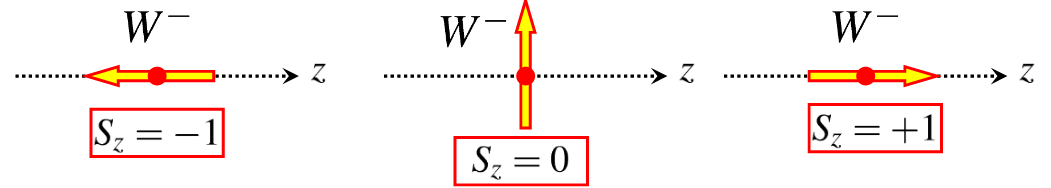
\includegraphics[width=\linewidth]{W_Polarization.png}
	\caption{The figure illustrates W-boson with negative, zero and positive
    helicity, corresponding to a left, longitudinal and right handed
    polarization. The right handed polarization will be heavily suppressed
    because of the (V-A) structure of the Wtb vertex.}\label{figpolarization}
\end{figure}

The fraction of; longitudinally $F_0$, left $F_L$ or right $F_R$ polarized
$W-$bosons which are produced from top quark decay, we refer to as helicity
fractions. In the Standard Model we can determine these fractions with quantum
chromo dynamics, in next to next to leading order (NNLO) calculations to be
$F_0 = 0.687 \pm 0.005$, $F_L = 0.311 \pm 0.005$ and
$F_R = 0.0017 \pm 0.0001$\cite{Czarnecki_2010}. The experimental method to
extract these fractions is by studying the angular decay distribution of the
leptonic decay products of the top quark. The angular distribution is given by:

\begin{equation}
  \frac{1}{\Gamma}\dv{\Gamma}{\cos \theta^*} = \frac{3}{8}(1-\cos \theta^*)^2 F_L +
  \frac{3}{4}\sin^2 \theta^* F_0 + \frac{3}{8}(1+\cos \theta^*)^2 F_R.
\end{equation}

Where $\theta^*$ is the helicity angle, which is defined as the angle between the
decayed lepton momentum direction, and the reversible momentum direction of the
$b$-quark decay from the same top quark, viewed from a reference frame with $W$
at rest\cite{PhysRevD.45.124}. From the 4-vectors of the lepton and $b$-jet, we
can find the $\cos \theta^*$ from the following expression:
\begin{equation}
  \frac{2 M_{eb}^2}{m_t^2 - M_W^2} - 1, \label{eq:costheta}
\end{equation}

here $p_l$ and $p_b$ are the four momentum vectors of the lepton and the bottom
quark respectively. $M_{lb}$ is the invariant mass of the lepton and bottom
quark system. The dependence is shown in Fig.~\ref{figdistributions} for the three
distribution seperately, and for the SM, with the above mentioned NNLO helicity
fractions.
\begin{figure}[H]
	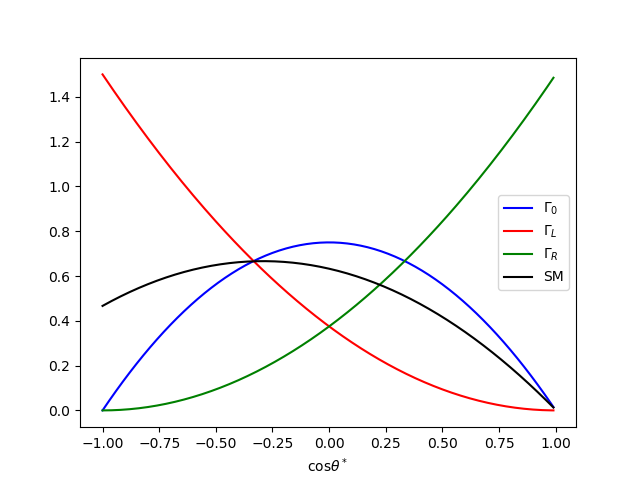
\includegraphics[width=\linewidth]{angular_dist.png}
	\caption{The predicted $\cos \theta^{*}$ angular distribution for helicity
    fractions. The distributions for $F_{0}$, $F_{L}$ and $F_{R}$ are
    normalized, and are given by the blue, red and green line respectively. The
    black line is the sum of the three contributions, but with helicity
    fractions given according to SM predictions.}\label{figdistributions}
\end{figure}

Another approach to obtaining the polarization states the $W$-bosons, is done by
counting the number of events with a specific $\cos \theta^*$, then use angular
asymmetries, $A_-$, and $A_+$, defined as
\begin{equation}
  A_{\pm}=\frac{N(\cos \theta^* > z)-N(\cos \theta^* < z)}{N(\cos \theta^* > z)+N(\cos \theta^* < z)},
\end{equation}

with $z=\pm(2^{2/3}-1)$, to choose asymmetries involving only dependence on
$F_0$ and $F_L$ for $A_+$, or $F_0$ and $F_R$ for $A_-$. The helicity fractions
for the $W$ boson, can then be obtained by,
\begin{align}
  F_R&=\frac{1}{1-\beta}+\frac{A_- - \beta A_+}{3\beta (1-\beta^2)},\\
  F_L&=\frac{1}{1-\beta}-\frac{A_+ - \beta A_-}{3\beta (1-\beta^2)},\\
  F_0&=-\frac{1+\beta}{1-\beta}+\frac{A_+ - A_-}{3\beta (1-\beta)},
\end{align}

where $\beta = 2^{1/3}-1$. The values for angular asymmetries is calculated in SM
NNLO as $A_+=0.537 \pm 0.004$ and $A_-=-0.841 \pm 0.006$.
%kilde findes på forsøgs artiklen.

\section{Apparatus}

\subsection{LHC}
In the Large Hadron Collider, top quarks are mainly produced through violent
collisions of protons, causing gluon-gluon fusion, which produces top, anti-top
pairs $gg \rightarrow t\bar t$. The data used in this paper, is from the 2016 run at LHC,
with a centre-of-mass energy of $\sqrt s = 13 \mathrm{TeV}$, which corresponds
to an integrated luminosity of 10 $\mathrm{fb}^{-1}$\cite{oreach2020}. At these
energies, the protons are accelerated close to the speed of light before their
collisions in the ATLAS detector.\\

This process starts, when protons are generated from an ion source in the linear
accelerator, LINAC2, then gets injected into the LHC, through a series of
smaller synchrotron accelerators, Proton Syncrotron Booster (PSB), Proton
Syncrotron (PS) and Super Protron Synhrotron (SPS)\cite[135]{Evans_2008}. The
LHC receives bunches from another SPS, containing a lot of protons in each
bunch, effectively increasing the cross-sectional area for collisions to occur.
In order to prevent energy loss due to synchrotron radiation, the LHC was built
to be the largest particle accelerator in the world, which has allowed it to
reach higher energies than other accelerators. At these energies, more events
happen inside the detector, described by the following equation:
\begin{equation}
  N = \sigma \int L \dd t,
\end{equation}

where $N$ is the number of expected events, $\sigma$ is the cross-sectional area of
the events, and $\int L \dd t$ is the integrated luminosity.
% Cern Thesis af Satoshi Hasegawa
%http://opendata.atlas.cern/release/2020/documentation/datasets/files.html

\subsection{ATLAS}
% https://atlas.web.cern.ch/Atlas/TP/NEW/HTML/tp9new/tp9.html
% https://atlas.cern/discover/detector
% https://en.wikipedia.org/wiki/ATLAS_experiment#ATLAS_detector
% Gamle hjemmeside: https://web.archive.org/web/20110614103207/http://atlas.ch/detector.html

% potential figure https://commons.wikimedia.org/wiki/File:ATLAS_Drawing.jpg

The ATLAS detector consists of multiple primary components, each with their own
subcomponents or subsections.

\subsubsection{The Inner Detector}
% https://atlas.web.cern.ch/Atlas/TP/NEW/HTML/tp9new/node10.html#SECTION00433000000000000000
% https://atlas.cern/discover/detector/inner-detector
% https://en.wikipedia.org/wiki/ATLAS_experiment#Inner_Detector

The purpose of this component is to measure charge and momentum, including it's
direction, of the detected particle. It consists of three subcomponents. 
\paragraph{Pixel Detector}
% https://iopscience.iop.org/article/10.1088/1748-0221/3/07/P07007
The pixel detector consists of approximately 92 million electronic channels. It's used for identification and reconstruction of secondary vertices from decay of particles containing a b-quark or for b-tagging jets. The pixel detector covers pseudorapidity range $|\eta| < 2.5 $ 
% Og mange flere kriterier relevant? 

\paragraph{Semiconductor Tracker}
%https://cds.cern.ch/record/1019885/files/indet-pub-2007-007.pdf
The Semiconductor tracker is a silicon microstrip tracker consisting of 4088 two-sided modules and over 6 million readout strips. These readout strips are distributed every $80\mathrm{\mu m}$ which allows recording of the position of charged particles to an accuracy of  $17\mathrm{\mu m}$

\paragraph{Transition Radiation Tracker.}
The transition radiation tracker is a drift tube tracker which consists of a straw of 4mm diameter and 0.03mm diameter tungsten wire coated with 0.5-0.7mm gold. The tube is filled with a gas mixture of Xe, $\mathrm{CO_{2}}$ and $\mathrm{O_{2}}$. When charged particles travel through the tube the gas gets ionized which frees electrons that move to the gold wire. The negative charge measured on the wire can be used to distinguish which charged particle ionized the gas. 
%Kringlet, probably  omskriv?

\subsubsection{Calorimeter}
% https://atlas.web.cern.ch/Atlas/TP/NEW/HTML/tp9new/node9.html#SECTION00432000000000000000
% https://atlas.cern/discover/detector/calorimeter
% https://en.wikipedia.org/wiki/ATLAS_experiment#Calorimeters
Calorimeters measure the energy of particles by absorbing them. There are two types of calorimeters used in ATLAS, the Electromagnetic Calorimeter (ECal) and Hadronic Calorimeter (HCal). ECal measures charged particles and photons. 
%Maybe Expand

The HCal consist of scintillator plates that radiates light when exposed to a charged particle. When a hadron passes through a scintillator plate it produces a shower of particles which then makes the scintillator radiate light. The intensity of the radiated light can then be analysed to measure the energy of the hadron.


\subsubsection{Muon Spectrometer}
% https://atlas.web.cern.ch/Atlas/TP/NEW/HTML/tp9new/node11.html#SECTION00434000000000000000
% https://atlas.cern/discover/detector/muon-spectrometer
% https://en.wikipedia.org/wiki/ATLAS_experiment#Muon_Spectrometer

The muon spectrometer is on the outer part of the ATLAS detector it operates in the pseudorapidity range $|\eta| < 2.7$. Muons usually pass through the inner detector and the calorimeters undetected which is why the muon spectrometer is located on the outside as other particles will have been stopped earlier in the detector. The muon spectrometer consists of tubes much like the transition radiation tracker that contains a gold wire which is surrounded by a gas. When muons go through these tubes they interact with the gas and leave behind a trail of ions and electrons which drift towards the gold wire in the centre. By detecting the starting point of these trails and measuring the time it takes to reach the gold wire the position of the muon can then be determined. The Muon Spectrometer can be seen in figure \ref{detector}  


\subsubsection{Data Collection}
% https://atlas.web.cern.ch/Atlas/TP/NEW/HTML/tp9new/node12.html
% https://en.wikipedia.org/wiki/ATLAS_experiment#Data_systems
% https://atlas.cern/discover/detector/trigger-daq
The detector generates 60 terabytes of data per second from the 1.7 billion
collisions taking place in the detector in that time frame. However, only some of the raw data contain interesting characteristics. To make the data more manageable ATLAS uses a two-level trigger system to only save the most important data. The first part of the trigger system is hardware based and can at most save 100 000 events per second, which then gets passed on to the High-Level Trigger which is software based. After both triggers approximately 1000 events out of the initial 1.7 billion are saved for later analysis.  

\begin{figure}[H]
	\centering
	\includegraphics[scale=0.1]{figures/atlas.jpg}
	\caption{A computer generated image of the ATLAS detector \cite{}}
	%http://cdsweb.cern.ch/record/1095924
	\label{detector}
\end{figure}

\section{Monte Carlo Simulation}
Monte Carlo (MC) simulation was used to model the signal and background
processes expected at the LHC, for the 13 TeV Atlas Open Data used for this
report. This process follows four steps, starting with an event generation which
uses a MC generator to mimic the initial pp collision. In the second step,
detector simulation, the geometry of the ATLAS detector and its material
properties gets simulated. As part of the digitisation step, the previous step
is followed by simulating the responding signals in read-out data written in a
format compatible with real output of the detector. Finally these data can be
used to reconstruct the collisions, particle trajectories and subsequent products.\\

In The 13 TeV ATLAS Open Data set, there are several SM processes which are
modelled using MC simulations. For the purpose of this report, the MC
simulations on top-quark-pair production was used alongside real data taken from
the detector, to compare theory with real data.
%http://opendata.atlas.cern/release/2020/documentation/datasets/mc.html

\section{Data Analysis}
% Definer Psuedorapidity \eta %
% http://opendata.atlas.cern/release/2020/documentation/physics/SL3.html
\subsection{Event Selection}
\label{sec:cuts}
In order to identify the top-quark-pair production, several cuts in the data
were implemented. The criteria are as follows \cite{oreach2020}
\begin{itemize}
	\item Only one electron or muon in the final state with $p_{T} > 30 \mathrm{GeV}$
	\item Missing transverse momentum $E_{T}^{miss} > 30 \mathrm{GeV}$
	\item Transverse mass of the W-boson $M_{T}^{W} > 30 \mathrm{GeV}$
	\item At least four jets with $p_{T} > 30 \mathrm{GeV}$, with exactly two of these being b-tagged
	\item Electrons are required to have $|\eta| > 2.47$ aside from $1.37 < |\eta| < 1.52$
	\item Muons are limited by $|\eta| > 2.50$
\end{itemize}
where $\eta$ describes angle between the particle and the beam axis given by 
\begin{equation}
	\eta = -\ln({\tan\left(\frac{\theta}{2}\right)})
\end{equation}

\subsubsection{B-tagging}
To study the $Wtb$ structure, a mechanism to identify the $b$-jets from the
other detected jets is required. First the jets are detected, $b$-hadrons,
$c$-hadrons or light-flavour jets, then their trajectories (tracks) are
reconstructed in the inner detector. Once a jet has been found, the jets
contining b-hadrons are then identified by a combination of three distinct
algorithms. Hadrons containing $b$-quarks have a long enough lifetime to fly a
measurable distance before it decays, and can be exploted to built
lifetime-based tagging algorithms. The impact parameter based algorithm, IP3D,
uses transverse and longitudinal impact parameter significances of each track
within a jet, the SV reconstructs the secondary vertex within the jet and decay
chain multi-vertex algorithm (JetFitter) reconstructs the full b-hadron
decay chain.\\

To better discriminate between jets, a Boosted Decision Tree (BDT) algorithm
called MV2c10, which uses the Root Toolkit for Multivariate Data Analysis
(TMVA), is used to make cuts that discards most of the background components,
the $c$- and light-flavoured jets. For this report, a $b$-jet efficiency rate of
70\% is used, which corresponds to a BDT cut value of 0.8244. This efficiency
rate originates from samples of simulated $t\bar t$ events with a $c$- and
light-jet rejection factor of nearly 400\cite{ATL-PHYS-PUB-2016-012}. At these
cuts, most of the $c$-jets and light-flavoured jets gets rejected, while still
maintaining most of the $b$-jet data.

%\subsubsection{Single Lepton Channel}

\subsection{Histograms from the ATLAS data}
After we have identified top-quark pair production we know that only one lepton
should be present in the event. This means that we can use the first lepton in
the event as the leading lepton. This lepton, however, can be either a electron
or a muon. Using this information we can construct the Lorentz vector for the
lepton, and from this we can plot the transverse energy.
% The function, which we use to construct the Lorentz vector, \texttt{SetPtEtaPhiE} is defined as such,
%\begin{equation}
%  p(pt, \eta, \phi, E) =
%  \begin{pmatrix}
%    |pt| \cos(\phi)\\ |pt|\sin(\phi)\\ |pt| \sinh(eta)\\ E
%  \end{pmatrix}
%\end{equation}
To calculate the
transverse energy we are using the builtin ROOT \texttt{TLorentzVector} member
function \texttt{Et()}. That function is effectively defined as
\begin{equation}
  % {{{\it p\_t}\,\sqrt{{\it p\_y}^2+{\it p\_x}^2}}\over{\sqrt{ {\it p\_z}^2+{\it p\_y}^2+{\it p\_x}^2}}}
  E_t = p_t \frac{\sqrt{p_y^2+p_x^2}}{\sqrt{p_z^2+p_y^2+p_x^2}}
\end{equation}
\begin{figure}[H]
  \centering
  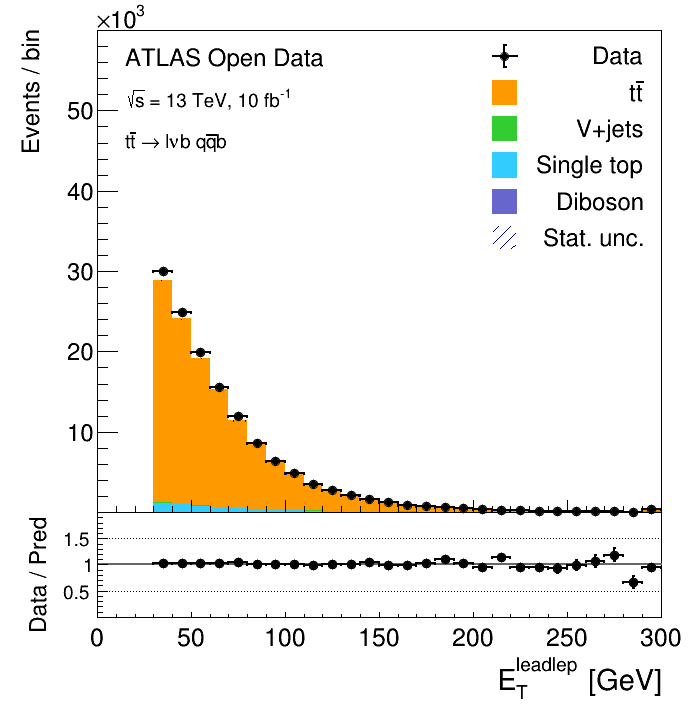
\includegraphics[width=0.55\textwidth]{figures/hist_leadleptEt}
  \caption{\label{fig:lepEt}Lead lepton transverse energy for both single-electron and single-muon channel.}
\end{figure}
% Wait, er det her ikke det samme da M er tæt på nul? Det er måske derfor de
% splitter electron muon. det kan være vi bare skal plotte noget andet eller vi
% kan jo selvfølgelig også bare gøre det samme som de gør ved at splitte
% electron/muon. Vi kan endda også bare plotte histogrammet med partikel id for
% at vise hvor mange af hver der er
\begin{figure}[H]
  \centering
  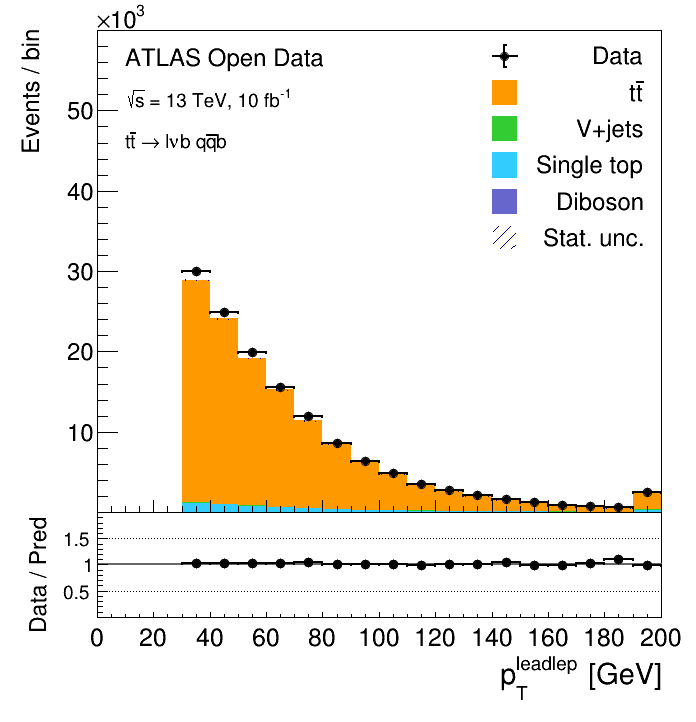
\includegraphics[width=0.55\textwidth]{figures/hist_leadleptpt}
  \caption{\label{fig:leppt}Lead lepton transverse momentum for both single-electron and single-muon channel.}
\end{figure}


In the given data we are directly given the missing transverse energy, which we
can then immediately plot if the given event satisfies all the criteria given in
subsection \ref{sec:cuts}. It is worth noting that it is given in the unit MeV, and all we have
to do is simply convert to GeV, for a more manageable unit in the plot.
\begin{figure}[H]
  \centering
  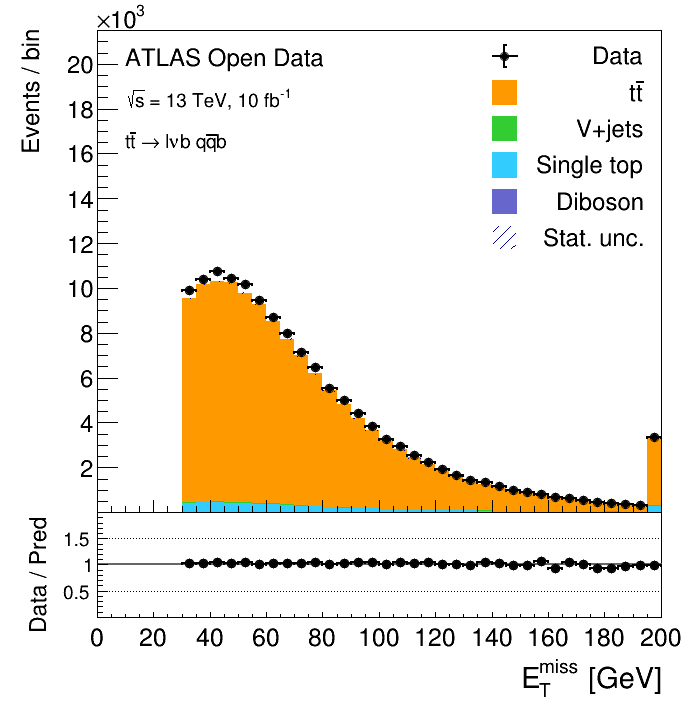
\includegraphics[width=0.55\textwidth]{figures/hist_etmiss}
  \caption{\label{fig:etmiss}Missing transverse energy for both single-electron and single-muon channel.}
\end{figure}

We are also given transverse momentum of jets in the event. % maybe explain jvt
The jets in the event are ordered and we can therefore get information about the
leading jet by accessing the first one. % also a requirement on pseudorapidity
% of the jets to be less than 2.5, however this should probably be mentioned in
% the criteria
\begin{figure}[H]
  \centering
  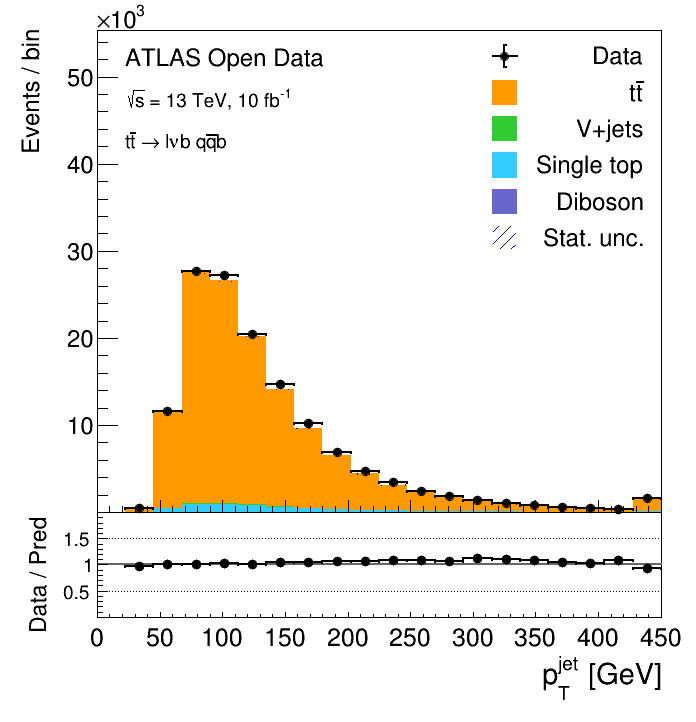
\includegraphics[width=0.55\textwidth]{figures/hist_leadjet_pt}
  \caption{\label{fig:jetpt}Lead jet transverse momentum for both single-electron and single-muon channel.}
\end{figure}



\subsection{$\cos \theta^{*}$ reconstruction}
From the data we can reconstruct $\cos \theta^{*}$ using equation \eqref{eq:costheta}.
\begin{figure}[H]
  \centering
  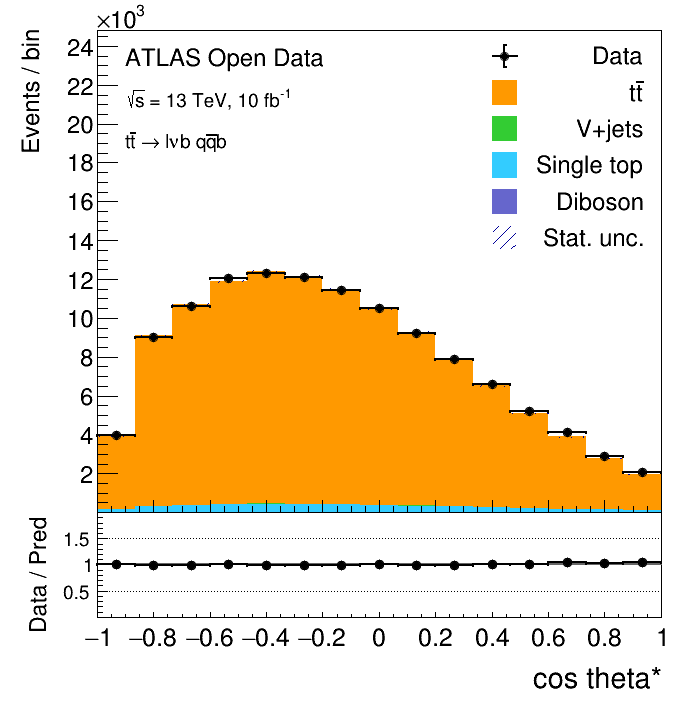
\includegraphics[width=0.6\textwidth]{figures/hist_costheta}
  \caption{\label{fig:costhetaatlas}Reconstructed $\cos \theta^{*}$ from ATLAS data.}
\end{figure}



% do we differentiate between them by S_z value
\subsection{Delphes data}
Using delphes we can at least verify that the generated data at least matches
the theoretical analytical functions plotted in figure \ref{figdistributions} as
a sanity check. % i guess we just fit them instead of doing
\begin{figure*}[t!]
    \centering
    \begin{subfigure}[t]{0.5\textwidth}
        \centering
        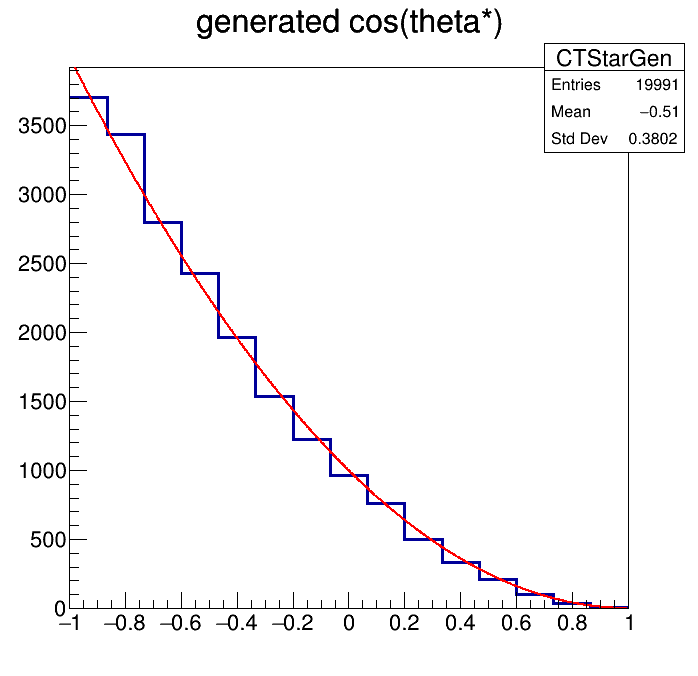
\includegraphics[width=1.0\textwidth]{figures/delphes_genL}
        \caption{Lorem ipsum}
    \end{subfigure}%
    \begin{subfigure}[t]{0.5\textwidth}
        \centering
        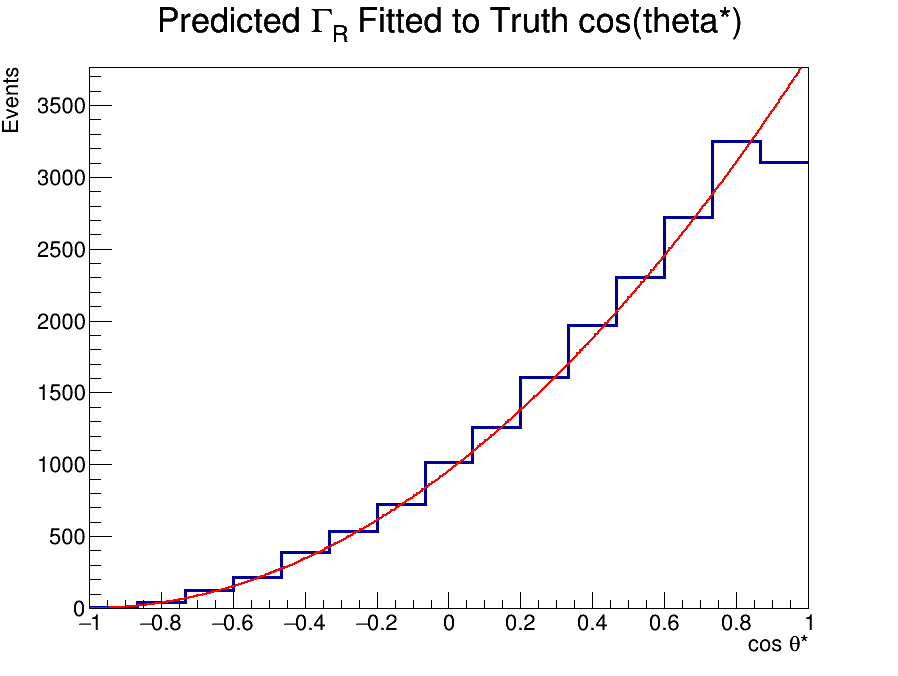
\includegraphics[width=1.0\textwidth]{figures/delphes_genR}
        \caption{Lorem ipsum, lorem ipsum,Lorem ipsum, lorem ipsum,Lorem ipsum}
      \end{subfigure}
    \begin{subfigure}[t]{0.5\textwidth}
        \centering
        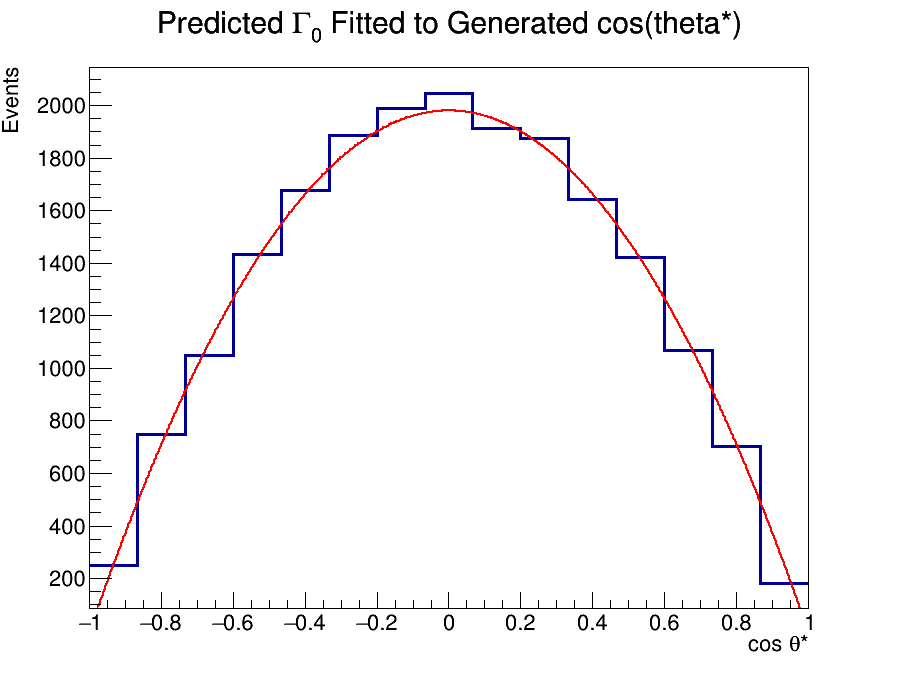
\includegraphics[width=1.0\textwidth]{figures/delphes_gen0}
        \caption{Lorem ipsum, lorem ipsum,Lorem ipsum, lorem ipsum,Lorem ipsum}
    \end{subfigure}
    \caption{Caption place holder}
\end{figure*}
Using the same information, as we would get in the ATLAS data, we can use the
same criteria from subsection \ref{sec:cuts} to isolate the equivalent usable
data, as we would get from the ATLAS detector, in the delphes data.
\begin{figure*}[t!]
    \centering
    \begin{subfigure}[t]{0.5\textwidth}
        \centering
        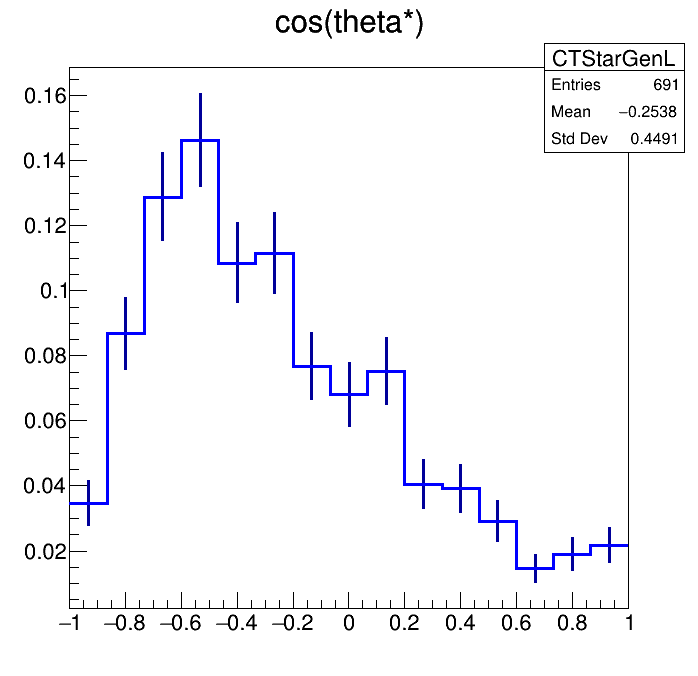
\includegraphics[width=1.0\textwidth]{figures/delphes_ctstarL}
        \caption{Lorem ipsum}
    \end{subfigure}%
    \begin{subfigure}[t]{0.5\textwidth}
        \centering
        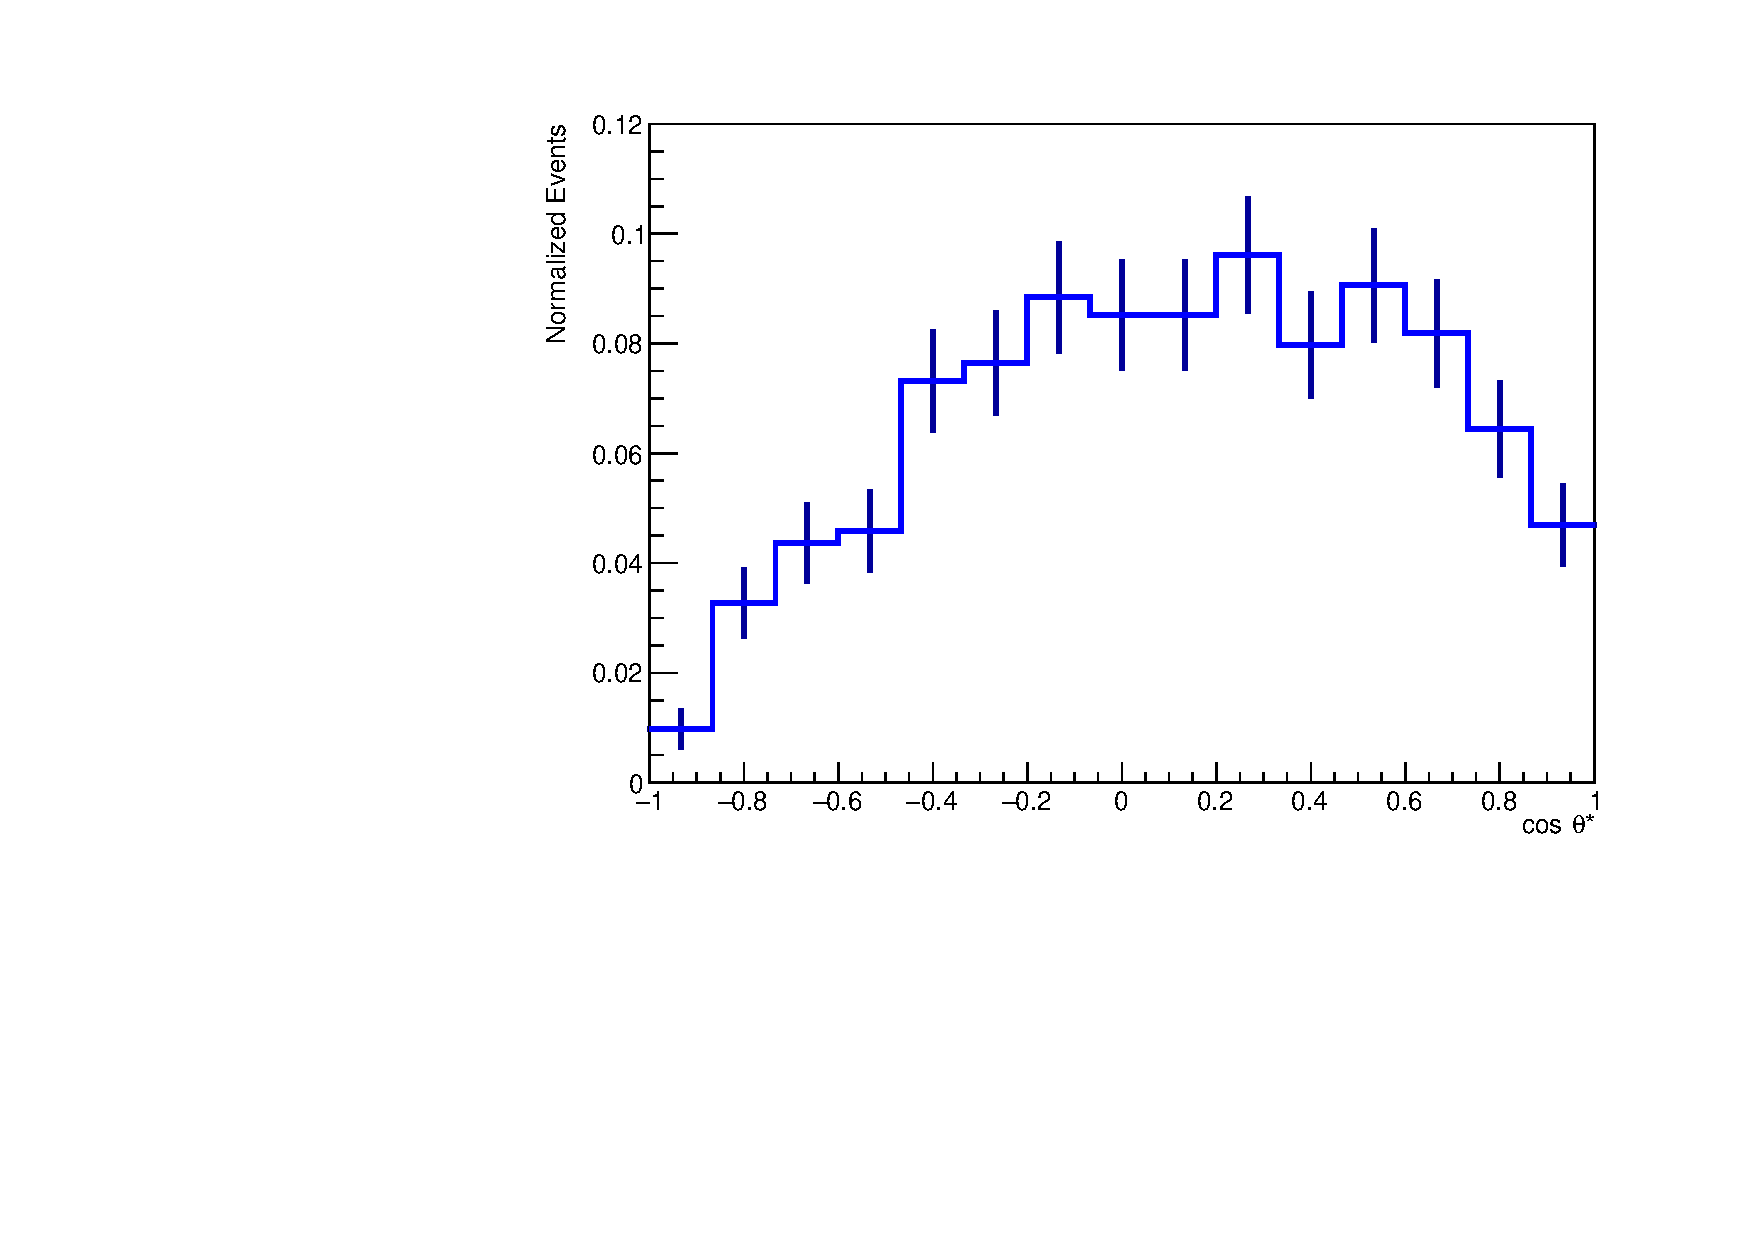
\includegraphics[width=1.0\textwidth]{figures/delphes_ctstarR}
        \caption{Lorem ipsum, lorem ipsum,Lorem ipsum, lorem ipsum,Lorem ipsum}
      \end{subfigure}
    \begin{subfigure}[t]{0.5\textwidth}
        \centering
        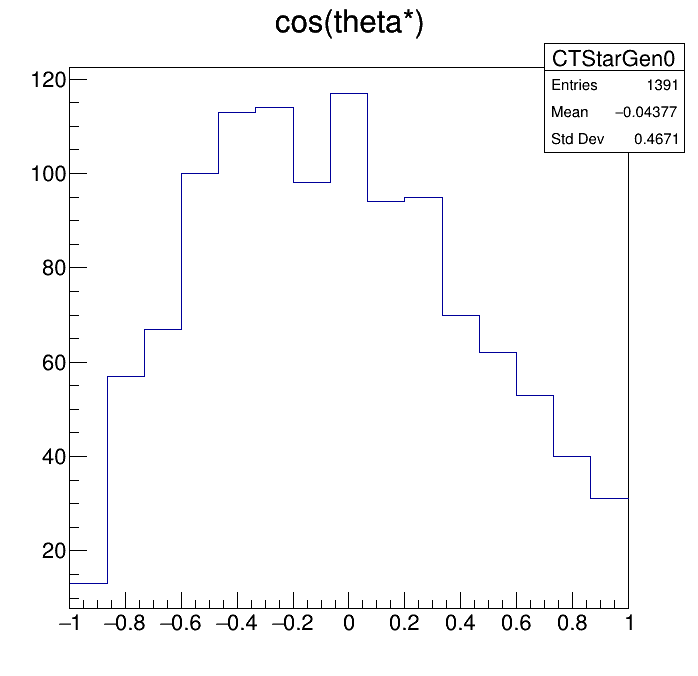
\includegraphics[width=1.0\textwidth]{figures/delphes_ctstar0}
        \caption{Lorem ipsum, lorem ipsum,Lorem ipsum, lorem ipsum,Lorem ipsum}
    \end{subfigure}
    \caption{Caption place holder}
\end{figure*}
We can now fit the resulting histograms in a linear combination to the histogram from the ATLAS data.
\cleardoublepage{}
\subsection{Fitting to atlas data}
\begin{figure}[H]
  \centering
  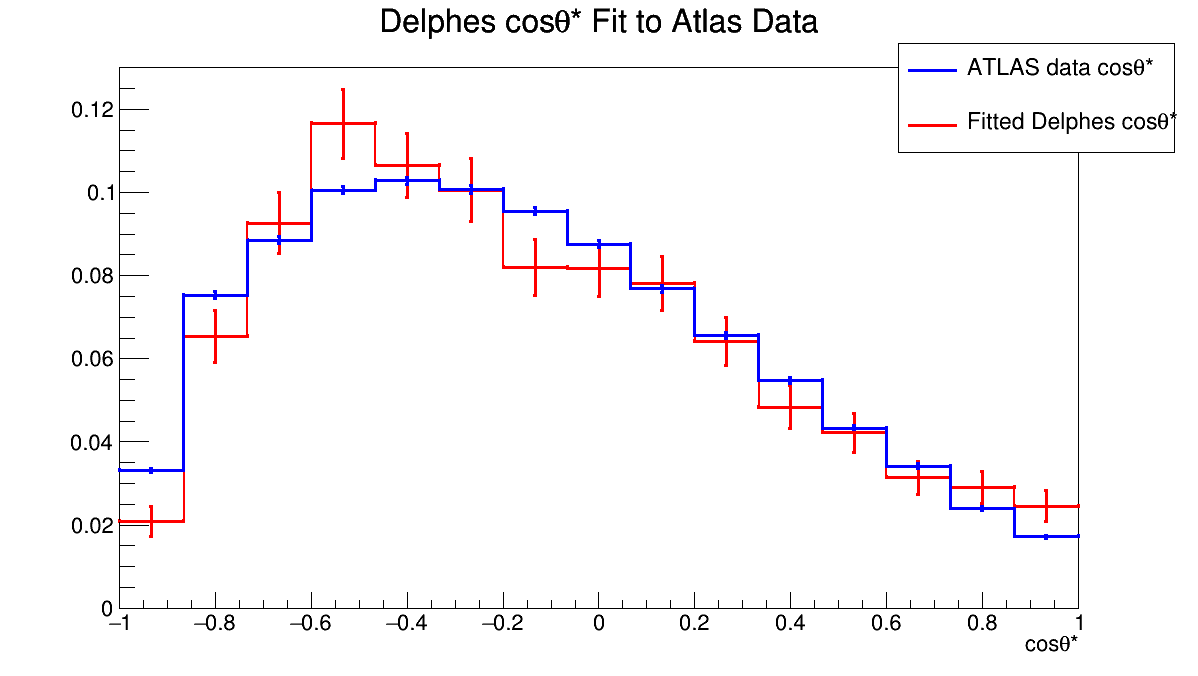
\includegraphics[width=0.6\textwidth]{figures/delphes_fit}
  \caption{\label{fig:delphesfit}Reconstructed Delphes $\cos \theta^{*}$ fitted to
    the $\cos \theta^{*}$ from ATLAS data.}
\end{figure}

\begin{verbatim}
FCN=954.777 FROM MIGRAD    STATUS=CONVERGED   217 CALLS   218 TOTAL
          EDM=3.15154e-10    STRATEGY= 1      ERROR MATRIX ACCURATE
 NO. PARAMETER VALUE         ERROR         STEP SIZE  FIRST DERIVATIVE
  1  F_0       4.00289e+01   1.28234e+00   4.79954e-03  -4.35846e-05
  2  F_L       2.79292e+01   4.50791e-01   3.37816e-03  -6.07790e-05
  3  F_R       2.28996e-01   4.03043e-01   2.22299e-03  -4.81292e-05
                               ERR DEF= 0.5
\end{verbatim}



%%% TODO: LAST of the four
%%% CHECK IF CHANNELS ARE WORTH DISTINGUISHING BETWEEN
%%% ADD COSTHETA
%%% DELPHES TRUTH
%%%




\subsection{The Code}

\subsubsection{ROOT}

\subsection{Results}

\section{Discussion}
Due to the limitations of the released 13 TeV Open Datasets, it was not possible
to analyse the helicity fractions angular distribution through that data, which
lead to the utilization of Delphes. The deviation between the predicted SM
values for the helicity fraction, and the value obtained through the fitting, is
possible the result of systematic errors in attempting to fit Delphes simulated
spin orientation, to the data obtained from the LHC Open ATLAS run in 2016.
Since Delphes runs a fast-simulation, it is not designed to be used in parallel
with data taken from advanced detector studies. This analysis consequently
serves as a test for this novel approach of combining Delphes simulations with
data taken from ATLAS detector. While similar cuts was attempted to be
implemented on the Delphes' truth-information, due to the absence of the
b-tagging MV2c10 algorithm in Delphes, cuts were made using 80\% efficiency
instead.\\  %skal finde en kilde til det her

The reconstructed $\cos \theta^*$ had significant entries in overflow. Attempts using
the theoretical $\cos \theta^*$, rather than the approximation, as seen in
Eq.~\ref{eq:costheta}, but no visible differences appeared, and the overflow
remained. This overflow was ignored in the fitting process, as only data
remaining within the physically possible range from -1 to 1, was considered in
the analysis. The Delphes data for the helicity destributions, had substantially
less overflow, than data from OpenATLAS, which also motived the decision to only
fit within the parameter -1 to 1.

\section{Conclusion}

\printbibliography

\end{document}
